
In this chapter, we will review several assumptions that are commonly used by various methods for estimating extinction times. In our review of these assumptions, we will also formulate two models that will be used by the methods discussed in the subsequent chapters. The most common assumptions seen are uniformity of fossil preservation and recovery; negligible radiometric error; and normally distributed radiometric errors.

\section{Uniformity Assumption}

A common approach is to assume that fossils are uniform and independently distributed over a fixed interval by representing the fossil recovery process by a homogeneous Poisson process. Implicitly, this also assumes that fossils are also perfectly preserved and recovered, which is generally not true as the abundance of a species can be expected to dwindle towards the beginning (speciation) and end (extinction) times \cite{Lee2010, WangMarshall2016}. 

Despite the consensus around the invalidity of assuming uniform fossil distribution, the majority of analyses to date continue to make this assumption. This is because ``first-generation" methods (a term coined by \citet{WangMarshall2016} identifying methods that make this uniformity assumption) of a lack of better alternatives: although methods that infer recovery rates from data exist, it is more often the case that the required quantitative knowledge of recovery rates are simply unavailable, making them inapplicable. Furthermore, the clarity, simplicity, and convenience of uniform assumptions allow ``first-generation" methods to persist in the literature.

\section{Negligible Measurement Error Assumption}

We first formulate a model under which we assume that fossils are generated by a homogeneous Poisson process and are therefore independently and uniformly distributed. We also assume negligible measurement error relative to other sources of variability, such as sampling error.

Let the true fossil dates be the random variables $\bm{X} = [X_1, \dots, X_n]^\top$, where $X_i$ is the number of years before present (BP). Let us also denote the fixed interval by $[\theta, K]$, where $\theta$ is the unknown parameter of interest, the extinction time, and $K$ is a known value representing a time at which we ``stop looking" for fossils. This may be interpreted as the speciation or invasion date; however, in practice, these dates are often unknown. As such, $K$ can be any arbitrarily selected upper bound as long as it is between the speciation date and extinction date.

A property of homogeneous Poisson processes is that the true fossil dates $\bm{X}$ are independent uniformly distributed random variables and the time gaps between fossil dates are exponentially distributed. We summarise this in the following model:
\begin{model}\label{model: no-measurement-error}
    Let the number of fossils be generated by a Poisson counting process with constant fossil recovery rate $\lambda$. Then:
    \begin{align*}
        n &\sim \textrm{Pois}(\lambda(K-\theta)) \\
        X_1, X_2, \dots, X_n  &\overset{i.i.d}{\sim} \mathcal{U}(\theta, K) \\
        G_i = X_i - X_{i+1} &\overset{i.i.d}{\sim} \exp{(\lambda)}
    \end{align*}
    for $i = 2, 3, \dots, n$, where $\theta$ is the unknown parameter of interest, $K$ is a known constant, and $G_i$ is the time gap between fossils.
\end{model}

This is the most direct and most common approach, with various methods in the literature making use of this assumption \cite{Strauss1989, Weiss1999, Solow1993, Mcinerny2006, Wang2016}. However, there is evidence to show this assumption is not generally applicable, as some fossil records will have dating errors that are comparable to the gaps between fossils \cite{Solow2006}. As such, this assumption should be checked prior to application of estimation methods.

\section{Measurement Error Assumption}

Next, we formulate a novel model under which measurement error is substantial and cannot be neglected, modifying Model \ref{model: no-measurement-error} to introduce measurement error. Let us now assume that the fossil ages $\bm{X}$ are now \textbf{unobserved} and have corresponding measurement errors $\bm{\varepsilon} = [\varepsilon_1, \dots, \varepsilon_n]^\top$, which are independently distributed according to a known density $f(e)$ with mean 0 and constant variance $\sigma^2$. Then, let the observed fossil ages be represented by $\bm{W} = \bm{X} + \bm{\varepsilon}$, which are truncated at the known upper bound $K$. This means the unobserved fossil ages $\bm{X}$ no longer need to be truncated at $K$, and so the upper bound for $\bm{X}$ is now $K-\bm{\varepsilon}$. Hence, we assume that $\bm{X}|\varepsilon$ is \textbf{conditionally uniform}:
\begin{model}\label{model: measurement-error}
    Let the number of fossils be generated by a Poisson counting process with constant fossil recovery rate $\lambda$. Then:
    \begin{align*}
        n &\sim \textrm{Pois}(\lambda(K-\theta)) \\
        X_i | \varepsilon_i &\overset{i.i.d}{\sim} \mathcal{U}(\theta, K-\varepsilon_i) \\
        \varepsilon_i &\overset{i.i.d}{\sim} f(e) \quad \E[\varepsilon] = 0, \Var(\varepsilon) = \sigma^2 \\
        W_i &= X_i + \varepsilon_i 
    \end{align*}
\end{model}

There are some additional nuances to this model. Since $X$ is greater than $\theta$ and $W$ must be less than $K$, $\varepsilon$ must therefore be less than $K - \theta$. This means that, in constructing a joint density for $(X, \varepsilon)$, we must also condition on $\varepsilon < K - \theta$ (see \autoref{fig: measurement-error-joint-density}). We will show how estimates of extinction times and confidence intervals can be constructed by exploiting these assumptions in our proposal of a novel method in \autoref{chap: proposed-methods}.
\begin{figure}[ht]
    \centering
    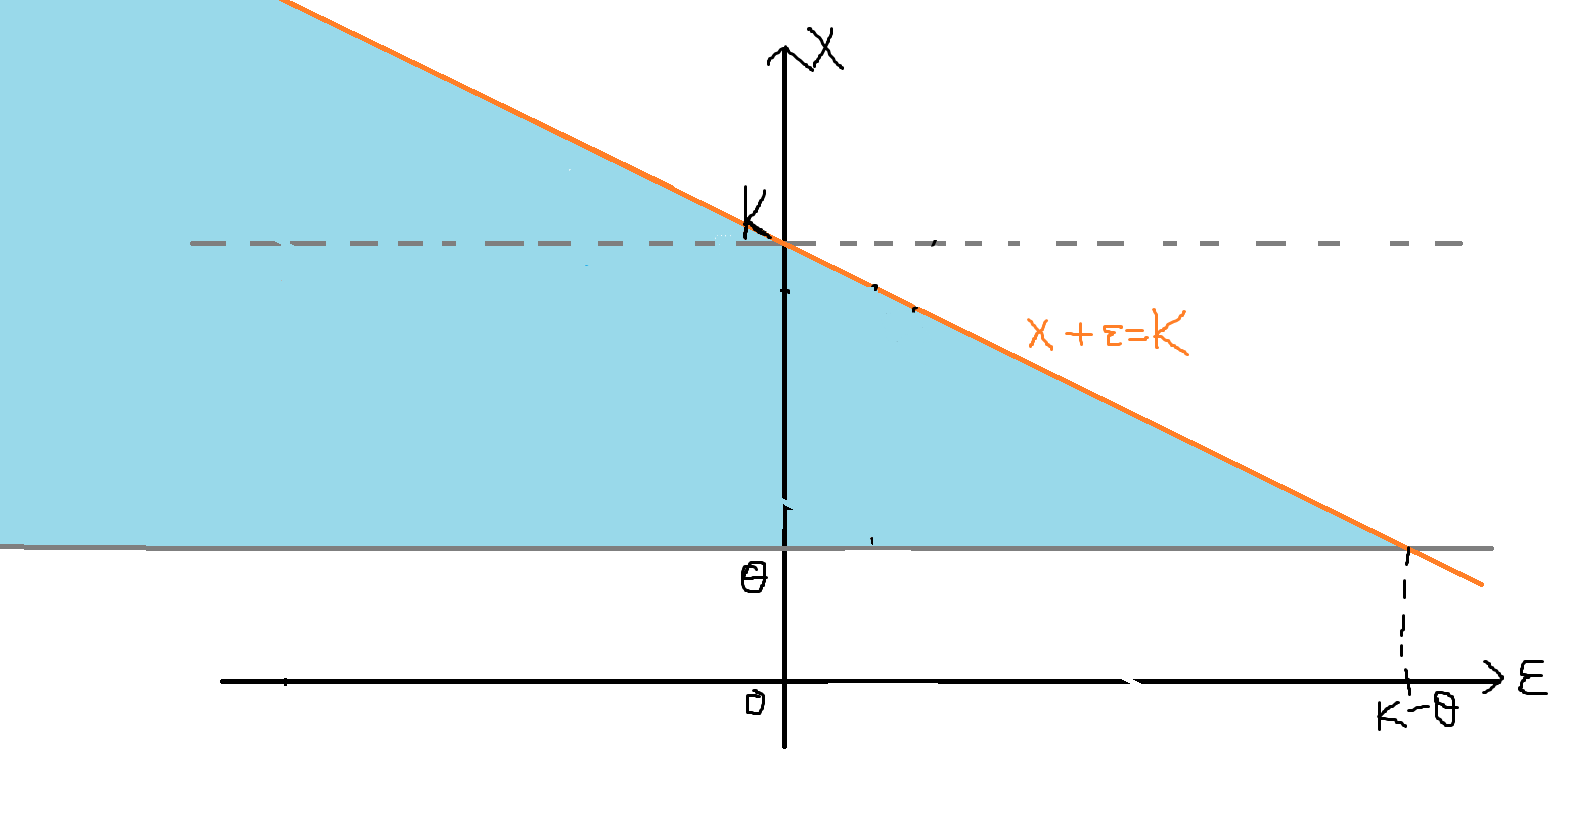
\includegraphics[width=0.8\textwidth]{figures/measurement-error-joint-density.png}
    \caption{Sketch of the region of the joint density $(X, \varepsilon)$, indicated by the shaded area. Note that it is bounded by the lines $X+\varepsilon = K$ and $X + \varepsilon = m$, and that the measurement errors are truncated at $K-\theta$.}
    \label{fig: measurement-error-joint-density}
\end{figure}

There still remains a question of how measurement errors are distributed. In this thesis, we will assume that $f(e)$ is normal and centered on zero with a constant $\sigma$ estimated from repeated radiometric  measurements and calibration. This is a fairly common approach in the literature: however, this model can be generalised to any a priori arbitrary measurement error distributions.

Assuming normally distributed radiometric errors is a common approach, as there is some evidence to show that radiocarbon dating errors are approximately normal \cite{Walker2005Quaternary}. However, although radiocarbon dating errors may be normally distributed (see panel 2 of \autoref{fig:variation_sources}), there is substantial evidence to suggest that the errors introduced by \textbf{calibration} curves are non normal (see panel 3 of \autoref{fig:variation_sources}). Moreover, since the same calibration curves are often used to calibrate the dates of fossils in the same dataset, these calibration errors may also be correlated \cite{Ramsey2009, Ramsey2010, Ramsey2013}.

\begin{figure}[ht]
    \centering
    \includegraphics[width=\linewidth]{figures/variation-sources-king.png}
    \caption{Sources of variation when estimating extinction times: 1. The sampling variation (note that the red line indicates the true extinction date and is past the last available fossil); 2. The radiocarbon dating measurement error, approximately normal in the figure; 3. The error introduced by the calibration process mapping radiocarbon dates to calendar dates. Reprinted from \citet{King2020}.}
    \label{fig:variation_sources}
\end{figure}
